                        %iffalse
                        \let\negmedspace\undefined
                        \let\negthickspace\undefined
                        \documentclass[journal,12pt,twocolumn]{IEEEtran}
                        \usepackage{cite}
                        \usepackage{amsmath,amssymb,amsfonts,amsthm}
                        \usepackage{algorithmic}
                        \usepackage{graphicx}
                        \usepackage{textcomp}
                        \usepackage{xcolor}
                        \usepackage{txfonts}
                        \usepackage{listings}
                        \usepackage{enumitem}
                        \usepackage{mathtools}
                        \usepackage{gensymb}
                        \usepackage{comment}
                        \usepackage[breaklinks=true]{hyperref}
                        \usepackage{tkz-euclide} 
                        \usepackage{listings}
                        \usepackage{gvv}                                        
                        %\def\inputGnumericTable{}    
                        \renewcommand{\thefigure}{\theenumi}
                        \renewcommand{\thetable}{\theenumi}
                        \usepackage[latin1]{inputenc}                                
                        \usepackage{color}                                            
                        \usepackage{array}                                            
                        \usepackage{longtable}                                       
                        \usepackage{calc}                                             
                        \usepackage{multirow}                                         
                        \usepackage{hhline} 
                        \usepackage{tikz}
                        \usepackage{ifthen}                                           
                        \usepackage{lscape}
                        \usepackage{tabularx}
                        \usepackage{array}
                        \usepackage{float}
                        \newtheorem{theorem}{Theorem}[section]
                        \newtheorem{problem}{Problem}
                        \newtheorem{proposition}{Proposition}[section]
                        \newtheorem{lemma}{Lemma}[section]
                        \newtheorem{corollary}[theorem]{Corollary}
                        \newtheorem{example}{Example}[section]
                        \newtheorem{definition}[problem]{Definition}
                        \newcommand{\BEQA}{\begin{eqnarray}}
                        \newcommand{\EEQA}{\end{eqnarray}}
                        \theoremstyle{remark}
                        % Marks the beginning of the document
                        \begin{document}
                        \bibliographystyle{IEEEtran}
                        \vspace{3cm}
                        \title{2021-March Session-03-18-2021-shift-2}
                        \author{AI24BTECH11006 - Bugada Roopansha}
                        \maketitle
                        \begin{enumerate}[start=69]
                        \item In a machine shop, pins of $15$ mm diameter are produced at a rate of $1000$ per month, and the same is consumed at a rate of $500$ per month. The production and consumption continue simultaneously till the maximum inventory is reached. Then inventory is allowed to reduce to zero due to consumption. The lot size of production is $1000$. If backlog is not allowed, the maximum inventory level is
                        \begin{enumerate}
                            \item $400$
                            \item $500$
                            \item $600$
                            \item $700$
                        \end{enumerate}
                        \item The net requirements of an item over $5$ consecutive weeks are $50-0-15-20-20$. The inventory carrying cost and ordering cost are Rs $\cdot1$ per item per week and Rs $\cdot100$ per order respectively. The starting inventory is zero. Use the least unit cost technique to develop the plan. The cost of the plan \brak{in Rs} is
                            \begin{enumerate}
                                \item $200$
                                \item $250$
                                \item $255$
                                \item $260$
                            \end{enumerate}
                        \section{Common Data for Questions$ 71, 72, 73$}    
					A gear set has a pinion with $20$ teeth and a gear with $40$ teeth. The pinion runs at $30 \frac{rev}{s}$ and transmits a power of $20$ kW. The teeth are on the $20^\circ$ full-depth system and have a module of $5$ mm. The length of the line of action is $19$ mm.
                            \item The center distance for the above gear set in mm is
                            \begin{enumerate}
                                \item $140$
                                \item $150$
                                \item $160$
                                \item $170$
                            \end{enumerate}
                            
                            \item The contact ratio of the contacting tooth is
                            \begin{enumerate}
                                \item $1.21$
                                \item $1.25$
                                \item $1.29$
                                \item $1.33$
                            \end{enumerate}
                            
                            \item The resultant force on the contacting gear tooth in N is
                            \begin{enumerate}
                                \item $77.23$
                                \item $212.20$
                                \item $225.80$
                                \item $289.43$
                            \end{enumerate}
                        \section{Common Data for Questions $74,75$}
                        A thermodynamic cycle with an ideal gas as working fluid is shown below.
                        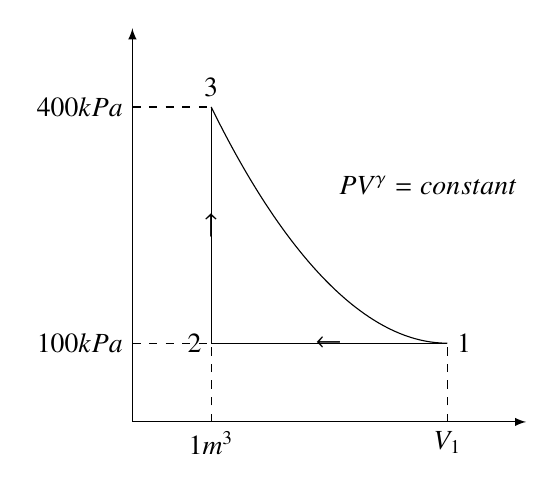
\begin{tikzpicture}
     \draw[->, >=latex] (0,0) -- (5,0);
     \draw[->, >=latex] (0,0) -- (0,5);
     \draw (1,1) -- (4,1)node[midway] {$\leftarrow$}node[right] at (4,1){$1$};
     \node[left] at (1,1){$2$};
     \draw (1,1) -- (1,4)node[midway] {$\uparrow$}node[above] at (1,4){$3$};
     \draw (4,1) parabola (1,4);
     \draw[dashed] (1,0) -- (1,1);
     \draw[dashed] (0,1) -- (1,1);
     \draw[dashed] (0,4) -- (1,4);
     \draw[dashed] (4,0) -- (4,1);
     \node[below] at (1,0){$1m^3$};
     \node[below] at (4,0){$V_1$};
     \node[left] at (0,1){$100kPa$};
     \node[left] at (0,4){$400kPa$};
     \node[left] at (5,3){$PV^\gamma=constant$};
\end{tikzpicture}
                        
                        \item The above cycle is represented on T-S plane by
                        \begin{enumerate}
                            \item \begin{tikzpicture}
     % Axes
    \draw[thick,->] (0,0) -- (4,0) node[right] {$S$};
    \draw[thick,->] (0,0) -- (0,4) node[above] {$T$};
    
    % Labels for points
    \node[left] at (1,1.5) {$1$};
    \node[right] at (3.2,0.75) {$2$};
    \node[above] at (1,3) {$3$};
    
    % Curves
    \draw (1,1.5) to(1,3);
    \draw (3.2,0.75) parabola (1,1.5);
    \draw (3.2,0.75) parabola (1,3);
\end{tikzpicture}
                             \item \begin{tikzpicture}
    % Axes
    \draw[thick,->] (0,0) -- (4,0) node[right] {$S$};
    \draw[thick,->] (0,0) -- (0,4) node[above] {$T$};
    
    % Labels for points
    \node[above] at (1.5,3) {$1$};
    \node[right] at (3,0.5) {$2$};
    \node[above] at (0.5,3) {$3$};
    
    % Curves
    \draw (0.5,3) to (1.5,3);
    \draw (3,0.5) parabola (0.5,3);
    \draw (3,0.5) parabola (1.5,3);
    
   
\end{tikzpicture}
                              \item \begin{tikzpicture}
    % Axes
    \draw[thick,->] (0,0) -- (4,0) node[right] {$S$};
    \draw[thick,->] (0,0) -- (0,4) node[above] {$T$};
    
    % Labels for points
    \node[below] at (3,1.5) {$1$};
    \node[left] at (1,1) {$2$};
    \node[above] at (3,3) {$3$};
    
    % Curves
    \draw (3,1.5) to (3,3);
    \draw (1,1) parabola (3,3);
    \draw (1,1) parabola (3,1.5);
    
   
\end{tikzpicture}
                               \item \begin{tikzpicture}
    % Axes
    \draw[thick,->] (0,0) -- (4,0) node[right] {$S$};
    \draw[thick,->] (0,0) -- (0,4) node[above] {$T$};
    
    % Labels for points
    \node[right] at (3,3) {$1$};
    \node[left] at (1,1) {$2$};
    \node[left] at (2,3) {$3$};
    
    % Curves
    \draw (2,3) to (3,3);
    \draw (1,1) parabola (3,3);
    \draw (1,1) parabola (2,3);
    
   
\end{tikzpicture}
                        \end{enumerate}
                          \item If the specific heats of the working fluid are constant and the value of specific heat ratio $y$ is $1.4$, the thermal efficiency $\brak{\%}$ of the cycle is
                            \begin{enumerate}
                                \item $21$
                                \item $40.9$
                                \item $42.6$
                                \item $59.7$
                            \end{enumerate} 
                        \section{Statement for linked questions $76,77 $}
                        Consider a steady incompressible flow through a channel as shown below.
                        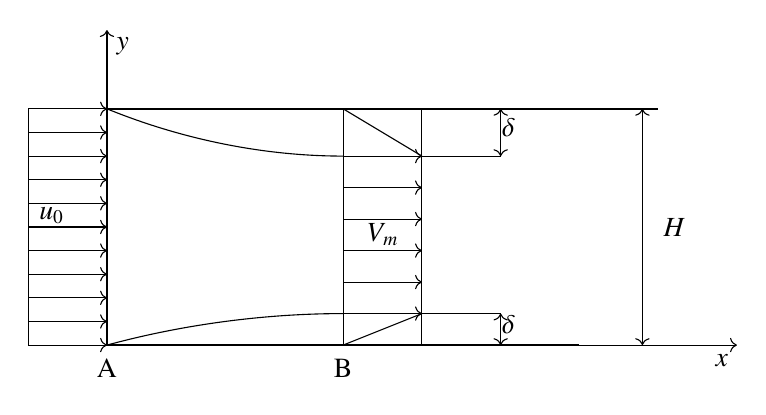
\begin{tikzpicture}

% Define coordinates for reference points A and B
\coordinate (A) at (0,0);
\coordinate (B) at (6,0);
\coordinate (C) at (0,3);
\coordinate (D) at (7,3);

% Add flow lines at inlet (uniform velocity profile at A)
\foreach \y in {0,0.3, 0.6, 0.9, 1.2, 1.5, 1.8, 2.1, 2.4, 2.7,3} {
    \draw[->] (-1,\y) -- (0,\y);
}
\foreach \y in {0.4, 0.8, 1.2, 1.6, 2, 2.4} {
    \draw[->] (3,\y) -- (4,\y);
}
% Label for u_0
\node at (-0.7, 1.65) {$u_0$};

% Draw flow lines along the channel and boundary layer growth
\foreach \x in {1.5, 3, 4.5} {
    
   
}

% Draw flow lines at B (developed profile)
\draw(3,2.4) parabola (0,3);
\draw(3,0.4) parabola (0,0);
\draw(-1,0) to (-1,3);
\draw(3,0) to (3,3);
\draw(4,0) to (4,3);
\draw(3,0) to (4,0.4);
\draw(3,3) to (4,2.4);
\draw(4,0.4) to(5,0.4);
\draw(4,2.4) -- (5,2.4);
% Boundary layer thickness labels
\draw[<->] (5,0) -- (5,0.4);
\draw[<->] (5,3) -- (5,2.4);
\node at (5.1,0.26) {$\delta$};
\node at (5.1,2.76) {$\delta$};

% Label for Vm (mean velocity)
\node at (3.5, 1.4) {$V_m$};

% Draw the height H between the plates
\draw[<->] (6.8,0) -- (6.8,3);
\node at (7.2,1.5) {$H$};

% Draw the plates
\draw[thick] (A) -- (B);
\draw[thick] (C) -- (D);

% Add x and y axes labels
\draw[->] (0,0) -- (0,4);
\node at (0.2,3.8) {$y$};

\draw[->] (-0.5,0) -- (8,0);
\node at (7.8,-0.2) {$x$};

% Labels for points A and B
\node at (0,-0.3) {A};
\node at (3,-0.3) {B};

\end{tikzpicture}

                        The velocity profile is uniform with a value of $u_o$ at the inlet section A. The velocity profile at section B downstream is
                        $$
                        u = 
                        \begin{cases} 
                        V_m\frac{y}{\delta} & \text{for}  0 \leq y \leq \delta \\ 
                        V_m & \text{for } \delta \leq y \leq H-\delta \\ 
                        V_m\frac{H-y}{\delta} & \text{for } H-\delta \leq y \leq H 
                        \end{cases}
                        $$
                            \item The ratio $\frac{V_m}{u_o}$ is
                            \begin{enumerate}
                                \item $\frac{1}{1 - 2\brak{\frac{\delta}{H}}}$
                                \item $1$
                                \item $\frac{1}{1 - \brak{\frac{\delta}{H}}}$
                                \item $\frac{1}{1 + \brak{\frac{\delta}{H}}}$
                            \end{enumerate}
                            
                            \item The ratio $\frac{P_A - P_B}{\frac{1}{2}\delta{u_o}^2}$ where $P_A$ and $P_B$ are the pressures at section A and B, respectively, and $\delta$ is the density of the fluid is
                            \begin{enumerate}
                                \item $ \frac{1}{\brak{1-\brak{\frac{\delta}{H}}}^2} -1$
                                \item $ \frac{1}{\brak{1-\brak{\frac{\delta}{H}}}^2}$
                                \item $ \frac{1}{\brak{1-\brak{\frac{2\delta}{H}}}^2} -1$
                                \item $ \frac{1}{1+\brak{\frac{\delta}{H}}}$
                            \end{enumerate}
                        \section{Statment for linked question $78 ,79$}
			Consider steady one-dimensional heat flow in a plate of $20$ mm thickness with a uniform heat generation of $80 \frac{MW}{m^3}$. The left and right faces are kept at constant temperatures of $160^\circ C$ and $120^\circ C$ respectively. The plate has a constant thermal conductivity of $200 \frac{W}{mK}$. 
                        
                        \item The location of maximum temperature within the plate from its left face is
                        \begin{enumerate}
                            \item $15$ mm
                            \item $10$ mm
                            \item $5$ mm
                            \item $0$ mm
                        \end{enumerate}
                            \item The maximum temperature within the plate in $^\circ C$ is
                            \begin{enumerate}
                                \item $160$
                                \item $165$
                                \item $200$
                                \item $250$
                            \end{enumerate}
                        \section{Statment for linked question $80,81$}
                        A machine frame shown in the figure below is subjected to a horizontal force of $600$ N parallel to z-direction.
                       \begin{tikzpicture}

% Define coordinates for reference points
\coordinate (P) at (0,0,0);  % Point P
\coordinate (top) at (0,3,0);  % Top of the vertical segment
\coordinate (end) at (5,3,0);  % End of the horizontal segment
\coordinate (base1) at (-2,-0.5,-2);  % Base corners


% Draw the base plate
\draw[thick] (base1) -- ++(0,0,4) -- ++(4,0,0) -- ++(0,0,-4) -- cycle;


% Draw the vertical segment (pipe)


% Draw the horizontal segment (pipe)


% Draw the 600 N force at the end of the pipe

% Labels and dimensions
\draw (-0.5,0,0) -- (-0.5,5,0);
\draw (0.5,0,0) -- (0.5,4.5,0);
\draw (6,5,0) -- (-0.5,5,0);
\draw (6,4.5,0) -- (0.5,4.5,0);
\draw (6,5.5,0) -- (-0.5,5.5,0) node[above,midway] {500mm};
\draw (-1,0,0) -- (-1,5,0)node[left,midway] {300mm};
\draw[->] (P) -- ++(0,7,0) node[above] {$y$};  % y-axis
\draw[->] (P) -- ++(5,0,0) node[right] {$x$};  % x-axis
\draw[->] (P) -- ++(0,0,4) node[below] {$z$};  % z-axis


% Label point P
\node at (-0.2,-0.2) {P};

\end{tikzpicture}
                        \item The normal and shear stresses in MPa at the point P are, respectively,
                        \begin{enumerate}
                            \item $67.9$ and $56.6$
                            \item $56.6$ and $67.9$
                            \item $67.9$ and $0.0$
                            \item $0.0$ and $56.6$
                        \end{enumerate}
                        \item  The maximum principal stress in MPa and the orientation of the corresponding principal plane in degrees are respectively
                            \begin{enumerate}
                               \item  $-32.0$ and $-29.52 $
                               \item  $100.0$ and $60.48 $
                               \item  $32.0$ and $60.48$ 
                               \item  $100.0$ and $-29.52$
                            \end{enumerate}
                        \section{Statement for linked questions$82 , 83$}
			  A quick return mechanism is shown below. The crank OS is driven at $2 \frac{rev}{s}$ in a counter-clockwise direction.
                        \begin{tikzpicture}

% Define coordinates
\coordinate (P) at (0,1);       % Point P
\coordinate (O) at (0,3);       % Point O (500 mm above P)
\coordinate (S) at (2,2.77);     % Point S (diagonal to O)
\coordinate (R) at (4.5,5);     % Point R (horizontal to O)
\coordinate (N) at (4,6.5);
% Draw the vertical wall
\draw[thick] (0,0) -- (0,5) node[midway, left] {}; % Wall from P to O
\draw[thick] (-3,6) -- (7,6) node[midway, left] {};
% Draw the beam OS
\draw[thick] (O) -- (S) node[midway, above right] {};  % Beam OS

% Draw the horizontal beam OR
\draw[thick] (P) -- (R) node[midway, above] {}; % Horizontal beam 
\draw[thick] (N) -- (R) node[midway, above] {};


% Points and labels
\filldraw[black] (P) circle (2pt) node[left] {P};  % Point P
\filldraw[black] (O) circle (2pt) node[left] {O};  % Point O
\filldraw[black] (S) circle (2pt) node[right] {S}; % Point S
\filldraw[black] (R) circle (2pt) node[right] {R}; % Point R
\filldraw[black] (N) circle (2pt) node[right] {N};
% Dimension line for PO (500 mm)
\draw[<->] (-0.5,1) -- (-0.5,3) node[midway, left] {500mm};
\draw (3.5,6) --(3.5,7) --(4.5,7) --(4.5,6);
% Angle indicator for the rotation at O
\draw[->] (0.3,2.5) arc[start angle=-60,end angle=0,radius=1] node[midway, right] {};

\end{tikzpicture}
                         \item If the quick return ratio is $1:2$, then the length of the crank in mm is
                            \begin{enumerate}
                               \item  $250$
                               \item  $250 \sqrt{3}$
                                \item $500$
                                \item $500 \sqrt{3}$
                            \end{enumerate}
		    \item The angular speed of PQ in $\frac{rev}{s}$ when the block R attains maximum speed during the forward stroke \brak{stroke with slower speed} is
                            \begin{enumerate}
                               \item  $\frac{1}{3}$
                               \item  $\frac{2}{3}$
                               \item  $2$
                               \item  $3$
                            \end{enumerate}
                            \section{Statement for linked questions$84 , 85$}
			 A low carbon steel bar of $147$ mm diameter with a length of $630$ mm is being turned with uncoated carbide insert. The observed tool lives are $24$ min and $12$ min for cutting velocities of $90 \frac{m}{min}$ and $120 \frac{m}{min}$ respectively. The feed and depth of cut are $0.2 \frac{mm}{rev}$ and $2$ mm respectively. Use the unmachined diameter to calculate the cutting velocity.
		 \item When tool life is $20$ min, the cutting velocity in $\frac{m}{min}$ is
                            \begin{enumerate}
                               \item  $87$ 
                               \item  $97$ 
                                \item $107$ 
                                \item $114$
                            \end{enumerate}
                        
                            \item Neglect over-travel or approach of the tool. When tool life is $20$ min, the machining time in min for a single pass is
                            \begin{enumerate}
                               \item  $5$
                                \item $10$ 
                                \item $15$ 
                                \item $20$
                            \end{enumerate}
                        \end{enumerate}
                        \end{document}
                        
